\documentclass[12pt, twoside]{article}
\usepackage[letterpaper, margin=1in, headsep=0.5in]{geometry}
\usepackage[english]{babel}
\usepackage[utf8]{inputenc}
\usepackage{amsmath}
\usepackage{amsfonts}
\usepackage{amssymb}
\usepackage{tikz}
\usetikzlibrary{quotes, angles}
\usepackage{graphicx}
\usepackage{enumitem}
\usepackage{multicol}
\usepackage{hyperref}

\newif\ifmeta
\metatrue %print standards and topics tags

\title{IB Mathematics}
\author{Chris Huson}
\date{January 2022}

\usepackage{fancyhdr}
\pagestyle{fancy}
\fancyhf{}
\renewcommand{\headrulewidth}{0pt} % disable the underline of the header
\raggedbottom


\fancyhead[LE]{\thepage}
\fancyhead[RO]{\thepage \\ Name: \hspace{4cm} \,\\}
\fancyhead[LO]{BECA / IB Math 03-Quadratic functions\\* 14 January 2022}

\begin{document}

\subsubsection*{3.7 Exit Note Quiz: Applications of quadratic functions}
\begin{enumerate}
\item A rectangular picture frame has a perimeter of 320 centimeters.
    \begin{enumerate}
        \item Let $x$ be the width of the frame in cm. Find an expression in terms of $x$ for the height of the frame. \vspace{2cm}
        \item Find an expression for the area of the frame, $A \,\rm{cm}^2$, in terms of $x$.  \vspace{2cm}
        \item Plot a graph of how the area varies with width. Mark the coordinates of the vertex and $x$-axis intercepts.
        \item Explain what the coordinates of the vertex represent in the context of the situation. \vspace{4cm}
    \end{enumerate}
    \begin{center}
    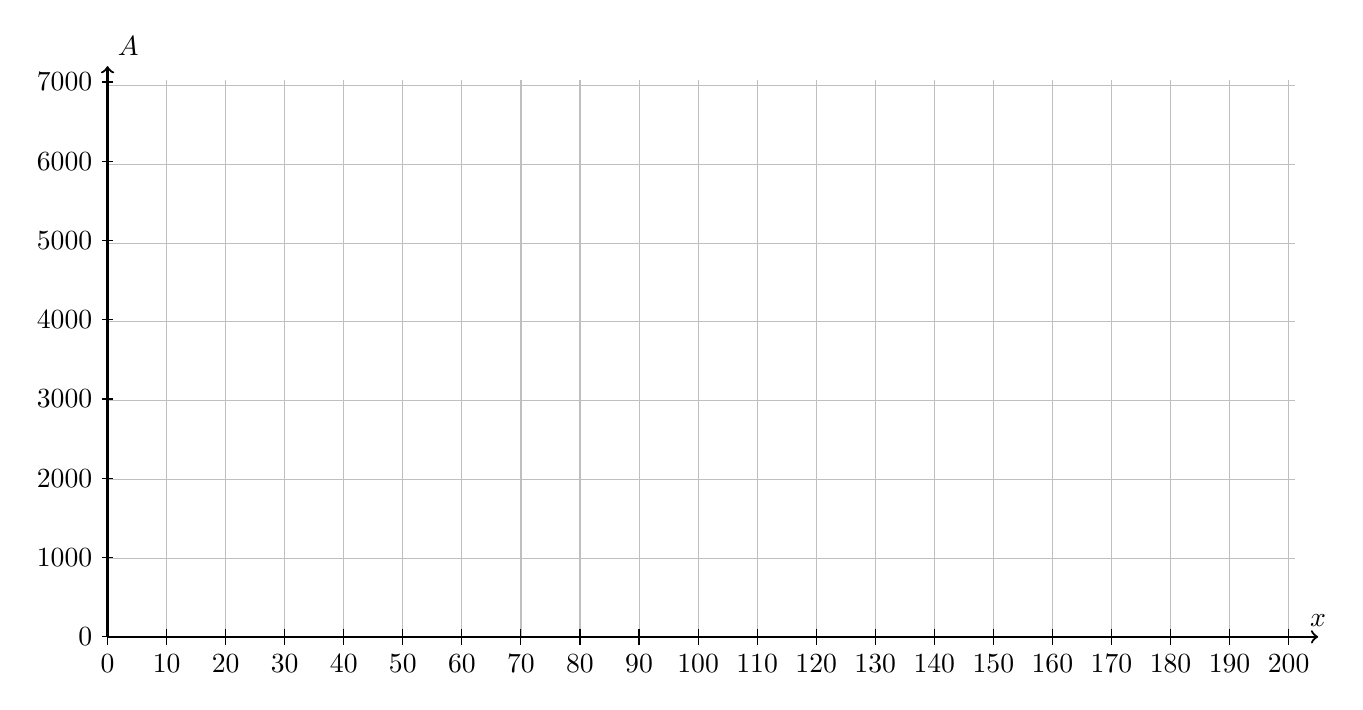
\begin{tikzpicture}[x=0.075cm, y=0.001cm]
        \draw [thin, color=lightgray, xstep=0.75cm,ystep=1.0cm] (0,0) grid (201,7020);
        \foreach \x in {0,10,...,200}
            \draw[shift={(\x,0)}] (0,3pt)--(0,-3pt) node[below]{$\x$};
        \foreach \y in {0,1000,...,7000}
            \draw[shift={(0,\y)}] (2pt,0pt)--(-2pt,0pt) node[left]{$\y$};
        \draw [thick, ->] (0,0) -- (+205,0) node [above] {$x$};
        \draw [thick, ->] (0,0) -- (0,7200) node [above right] {$A$};
        %\draw [thick, <->,smooth,domain=0:160] plot(\x,-\x*\x+160*\x);
    \end{tikzpicture}
    \end{center}
    
\newpage
Sum of an arithmetic series: $\displaystyle S_n=\frac{n}{2}(2u_1+d(n-1))$
\item The first four terms of an arithmetic sequence are 6, 10, 14, 18. 
\begin{enumerate}
    \item Write down the common difference, $d$. \vspace{0.5cm}
    \item Show the the sum to $n$ terms can be written as $2n^2+4n$.\vspace{3cm}
    \item The sum of $n$ terms is 880. Write a quadratic equation to represent this information. Rearrange to equal zero and plot the function, showing the $x$-intercepts and the coordinates of the vertex.\vspace{2cm}
    \item State what information the positive $x$-intercept tells you about the sequence.
\end{enumerate}
\vspace{3cm}
\begin{center}
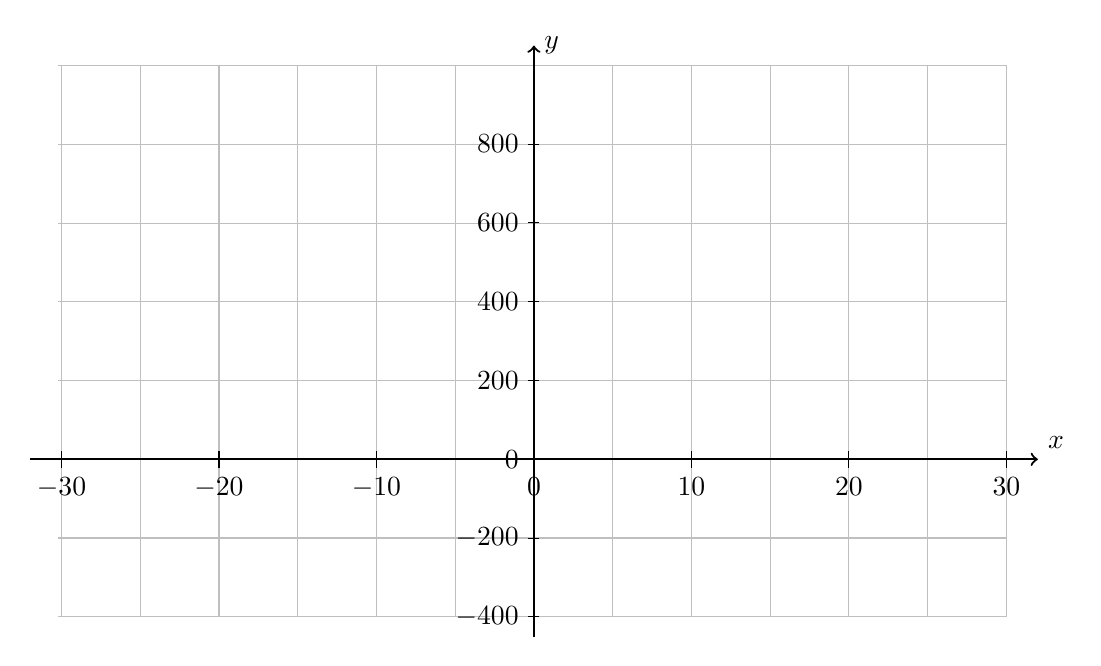
\begin{tikzpicture}[x=0.2cm, y=0.005cm]
    \draw [thin, color=lightgray, xstep=1.0cm,ystep=1.0cm] (-30.2,-400) grid (30,1000);
    \foreach \x in {-30,-20,...,30}
        \draw[shift={(\x,0)}] (0,3pt)--(0,-3pt) node[below] {$\x$};
    \foreach \y in {-400,-200,...,800}
        \draw[shift={(0,\y)}] (2pt,0pt)--(-2pt,0pt) node[left]  {$\y$};
    \draw [thick, ->] (-32,0) -- (+32,0) node [above right] {$x$};
    \draw [thick, ->] (0,-450) -- (0,1050) node [right] {$y$};
    %\draw [thick, <->,smooth,domain=-25:22] plot(\x,2*\x*\x+4*\x-880);
\end{tikzpicture}
\end{center}

\end{enumerate}
\end{document}